\documentclass{standalone}
\usepackage{tikz}
\usetikzlibrary{patterns, positioning}
\usepackage[sfdefault]{ClearSans} %% option 'sfdefault' activates Clear Sans as the default text font
\usepackage[T1]{fontenc}

\begin{document}
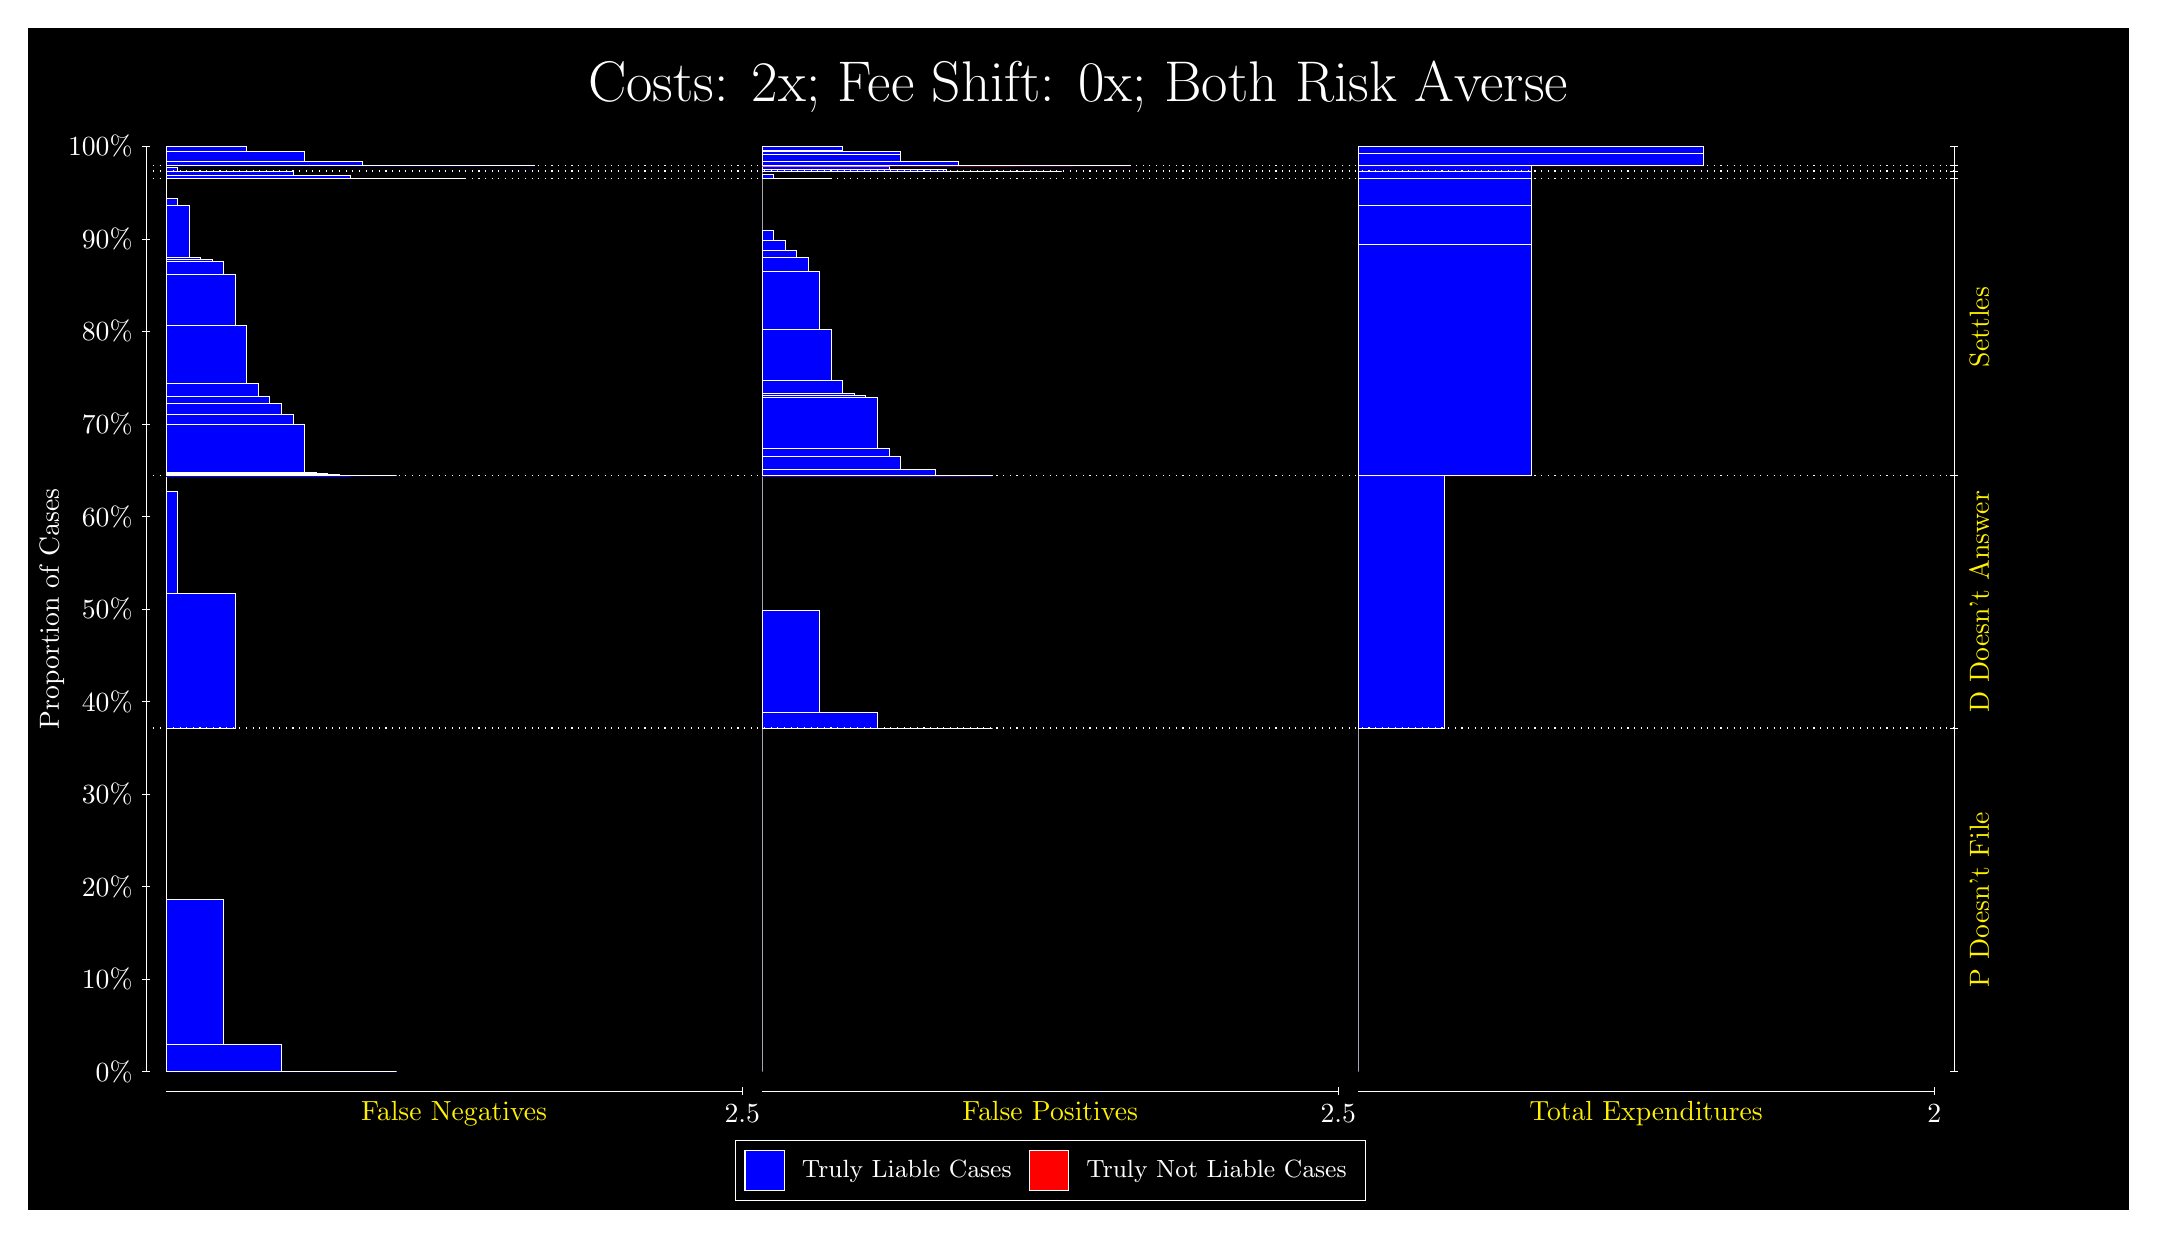
\begin{tikzpicture}
\draw[fill=black] (0,0) rectangle (26.667,15);
\draw[text=white] (0,13.5) rectangle (26.667,15) node[midway] {\huge Costs: 2x; Fee Shift: 0x; Both Risk Averse};
\draw[white, very thin] (1.5,1.75) -- (1.5,13.5);
\node[rotate=90, text=white, anchor=center] at (0.3, 7.625) {Proportion of Cases};
\draw[white, very thin] (1.45,1.75) -- (1.55,1.75);
\node[text=white, anchor=east] at (1.45, 1.75) {0\%};
\draw[white, very thin] (1.45,2.925) -- (1.55,2.925);
\node[text=white, anchor=east] at (1.45, 2.925) {10\%};
\draw[white, very thin] (1.45,4.1) -- (1.55,4.1);
\node[text=white, anchor=east] at (1.45, 4.1) {20\%};
\draw[white, very thin] (1.45,5.275) -- (1.55,5.275);
\node[text=white, anchor=east] at (1.45, 5.275) {30\%};
\draw[white, very thin] (1.45,6.45) -- (1.55,6.45);
\node[text=white, anchor=east] at (1.45, 6.45) {40\%};
\draw[white, very thin] (1.45,7.625) -- (1.55,7.625);
\node[text=white, anchor=east] at (1.45, 7.625) {50\%};
\draw[white, very thin] (1.45,8.8) -- (1.55,8.8);
\node[text=white, anchor=east] at (1.45, 8.8) {60\%};
\draw[white, very thin] (1.45,9.975) -- (1.55,9.975);
\node[text=white, anchor=east] at (1.45, 9.975) {70\%};
\draw[white, very thin] (1.45,11.15) -- (1.55,11.15);
\node[text=white, anchor=east] at (1.45, 11.15) {80\%};
\draw[white, very thin] (1.45,12.325) -- (1.55,12.325);
\node[text=white, anchor=east] at (1.45, 12.325) {90\%};
\draw[white, very thin] (1.45,13.5) -- (1.55,13.5);
\node[text=white, anchor=east] at (1.45, 13.5) {100\%};

\draw[white, very thin] (24.457,1.75) -- (24.457,13.5);
\draw[white, very thin] (24.407,1.75) -- (24.507,1.75);
\node[anchor=west] at (24.407, 1.75) {};
\draw[white, very thin] (24.407,6.1133) -- (24.507,6.1133);
\node[anchor=west] at (24.407, 6.1133) {};
\draw[white, very thin] (24.407,9.3165) -- (24.507,9.3165);
\node[anchor=west] at (24.407, 9.3165) {};
\draw[white, very thin] (24.407,13.092) -- (24.507,13.092);
\node[anchor=west] at (24.407, 13.092) {};
\draw[white, very thin] (24.407,13.186) -- (24.507,13.186);
\node[anchor=west] at (24.407, 13.186) {};
\draw[white, very thin] (24.407,13.253) -- (24.507,13.253);
\node[anchor=west] at (24.407, 13.253) {};
\draw[white, very thin] (24.407,13.5) -- (24.507,13.5);
\node[anchor=west] at (24.407, 13.5) {};

\draw[white, very thin, fill=blue] (1.75,1.75) rectangle (4.6775,1.75);
\draw[white, very thin, fill=blue] (1.75,1.75) rectangle (3.9457,1.7529);
\draw[white, very thin, fill=blue] (1.75,1.7529) rectangle (3.2138,2.0992);
\draw[white, very thin, fill=blue] (1.75,2.0992) rectangle (2.4819,3.9347);
\draw[white, very thin, fill=red] (1.75,3.9347) rectangle (1.75,3.9347);
\draw[white, very thin, fill=blue] (1.75,3.9347) rectangle (1.75,6.1133);
\draw[white, very thin, fill=blue] (1.75,6.1133) rectangle (2.6283,7.8263);
\draw[white, very thin, fill=blue] (1.75,7.8263) rectangle (1.8964,9.1141);
\draw[white, very thin, fill=red] (1.75,9.1141) rectangle (1.75,9.1141);
\draw[white, very thin, fill=blue] (1.75,9.1141) rectangle (1.75,9.3165);
\draw[white, very thin, fill=blue] (1.75,9.3165) rectangle (4.6775,9.3165);
\draw[white, very thin, fill=blue] (1.75,9.3165) rectangle (4.3848,9.3165);
\draw[white, very thin, fill=blue] (1.75,9.3165) rectangle (4.092,9.3168);
\draw[white, very thin, fill=blue] (1.75,9.3168) rectangle (3.9457,9.333);
\draw[white, very thin, fill=blue] (1.75,9.333) rectangle (3.7993,9.3539);
\draw[white, very thin, fill=blue] (1.75,9.3539) rectangle (3.6529,9.3623);
\draw[white, very thin, fill=blue] (1.75,9.3623) rectangle (3.5065,9.9759);
\draw[white, very thin, fill=blue] (1.75,9.9759) rectangle (3.3602,10.097);
\draw[white, very thin, fill=blue] (1.75,10.097) rectangle (3.2138,10.235);
\draw[white, very thin, fill=blue] (1.75,10.235) rectangle (3.0674,10.32);
\draw[white, very thin, fill=blue] (1.75,10.32) rectangle (2.921,10.495);
\draw[white, very thin, fill=blue] (1.75,10.495) rectangle (2.7746,11.228);
\draw[white, very thin, fill=blue] (1.75,11.228) rectangle (2.6283,11.875);
\draw[white, very thin, fill=blue] (1.75,11.875) rectangle (2.4819,12.044);
\draw[white, very thin, fill=blue] (1.75,12.044) rectangle (2.3355,12.065);
\draw[white, very thin, fill=blue] (1.75,12.065) rectangle (2.1891,12.095);
\draw[white, very thin, fill=blue] (1.75,12.095) rectangle (2.0428,12.745);
\draw[white, very thin, fill=blue] (1.75,12.745) rectangle (1.8964,12.842);
\draw[white, very thin, fill=red] (1.75,12.842) rectangle (1.75,12.842);
\draw[white, very thin, fill=blue] (1.75,12.842) rectangle (1.75,13.092);
\draw[white, very thin, fill=blue] (1.75,13.092) rectangle (5.5558,13.092);
\draw[white, very thin, fill=blue] (1.75,13.092) rectangle (4.8239,13.092);
\draw[white, very thin, fill=blue] (1.75,13.092) rectangle (4.092,13.127);
\draw[white, very thin, fill=blue] (1.75,13.127) rectangle (3.3602,13.185);
\draw[white, very thin, fill=blue] (1.75,13.185) rectangle (2.6283,13.186);
\draw[white, very thin, fill=red] (1.75,13.186) rectangle (1.75,13.186);
\draw[white, very thin, fill=blue] (1.75,13.186) rectangle (2.6283,13.187);
\draw[white, very thin, fill=blue] (1.75,13.187) rectangle (1.8964,13.228);
\draw[white, very thin, fill=red] (1.75,13.228) rectangle (1.75,13.228);
\draw[white, very thin, fill=blue] (1.75,13.228) rectangle (1.75,13.253);
\draw[white, very thin, fill=blue] (1.75,13.253) rectangle (6.4341,13.253);
\draw[white, very thin, fill=blue] (1.75,13.253) rectangle (5.7022,13.253);
\draw[white, very thin, fill=blue] (1.75,13.253) rectangle (4.9703,13.257);
\draw[white, very thin, fill=blue] (1.75,13.257) rectangle (4.2384,13.314);
\draw[white, very thin, fill=blue] (1.75,13.314) rectangle (3.5065,13.438);
\draw[white, very thin, fill=blue] (1.75,13.438) rectangle (2.7746,13.496);
\draw[white, very thin, fill=blue] (1.75,13.496) rectangle (2.0428,13.5);
\draw[white, very thin, fill=red] (1.75,13.5) rectangle (1.75,13.5);
\draw[white, very thin, fill=blue] (1.75,13.5) rectangle (1.75,13.5);
\draw[white, very thin, fill=red] (9.3189,1.75) rectangle (9.3189,1.75);
\draw[white, very thin, fill=blue] (9.3189,1.75) rectangle (9.3189,6.1133);
\draw[white, very thin, fill=red] (9.3189,6.1133) rectangle (12.246,6.1133);
\draw[white, very thin, fill=blue] (9.3189,6.1133) rectangle (12.246,6.1133);
\draw[white, very thin, fill=blue] (9.3189,6.1133) rectangle (11.515,6.1138);
\draw[white, very thin, fill=blue] (9.3189,6.1138) rectangle (10.783,6.3157);
\draw[white, very thin, fill=blue] (9.3189,6.3157) rectangle (10.051,7.6035);
\draw[white, very thin, fill=blue] (9.3189,7.6035) rectangle (9.3189,9.3165);
\draw[white, very thin, fill=red] (9.3189,9.3165) rectangle (12.246,9.3165);
\draw[white, very thin, fill=blue] (9.3189,9.3165) rectangle (12.246,9.3167);
\draw[white, very thin, fill=red] (9.3189,9.3167) rectangle (11.954,9.3167);
\draw[white, very thin, fill=blue] (9.3189,9.3167) rectangle (11.954,9.3167);
\draw[white, very thin, fill=red] (9.3189,9.3167) rectangle (11.661,9.3167);
\draw[white, very thin, fill=blue] (9.3189,9.3167) rectangle (11.661,9.3169);
\draw[white, very thin, fill=blue] (9.3189,9.3169) rectangle (11.515,9.398);
\draw[white, very thin, fill=red] (9.3189,9.398) rectangle (11.368,9.398);
\draw[white, very thin, fill=blue] (9.3189,9.398) rectangle (11.368,9.3983);
\draw[white, very thin, fill=blue] (9.3189,9.3983) rectangle (11.222,9.3983);
\draw[white, very thin, fill=red] (9.3189,9.3983) rectangle (11.075,9.3983);
\draw[white, very thin, fill=blue] (9.3189,9.3983) rectangle (11.075,9.566);
\draw[white, very thin, fill=blue] (9.3189,9.566) rectangle (10.929,9.6629);
\draw[white, very thin, fill=blue] (9.3189,9.6629) rectangle (10.783,10.313);
\draw[white, very thin, fill=blue] (9.3189,10.313) rectangle (10.636,10.344);
\draw[white, very thin, fill=blue] (9.3189,10.344) rectangle (10.49,10.365);
\draw[white, very thin, fill=blue] (9.3189,10.365) rectangle (10.344,10.534);
\draw[white, very thin, fill=blue] (9.3189,10.534) rectangle (10.197,11.18);
\draw[white, very thin, fill=blue] (9.3189,11.18) rectangle (10.051,11.913);
\draw[white, very thin, fill=blue] (9.3189,11.913) rectangle (9.9044,12.088);
\draw[white, very thin, fill=blue] (9.3189,12.088) rectangle (9.758,12.174);
\draw[white, very thin, fill=blue] (9.3189,12.174) rectangle (9.6116,12.312);
\draw[white, very thin, fill=blue] (9.3189,12.312) rectangle (9.4652,12.432);
\draw[white, very thin, fill=blue] (9.3189,12.432) rectangle (9.3189,13.092);
\draw[white, very thin, fill=red] (9.3189,13.092) rectangle (10.197,13.092);
\draw[white, very thin, fill=blue] (9.3189,13.092) rectangle (10.197,13.093);
\draw[white, very thin, fill=blue] (9.3189,13.093) rectangle (9.4652,13.151);
\draw[white, very thin, fill=blue] (9.3189,13.151) rectangle (9.3189,13.186);
\draw[white, very thin, fill=red] (9.3189,13.186) rectangle (13.125,13.186);
\draw[white, very thin, fill=blue] (9.3189,13.186) rectangle (13.125,13.186);
\draw[white, very thin, fill=blue] (9.3189,13.186) rectangle (12.393,13.186);
\draw[white, very thin, fill=blue] (9.3189,13.186) rectangle (11.661,13.211);
\draw[white, very thin, fill=blue] (9.3189,13.211) rectangle (10.929,13.252);
\draw[white, very thin, fill=blue] (9.3189,13.252) rectangle (10.197,13.253);
\draw[white, very thin, fill=red] (9.3189,13.253) rectangle (14.003,13.253);
\draw[white, very thin, fill=blue] (9.3189,13.253) rectangle (14.003,13.253);
\draw[white, very thin, fill=red] (9.3189,13.253) rectangle (13.271,13.253);
\draw[white, very thin, fill=blue] (9.3189,13.253) rectangle (13.271,13.253);
\draw[white, very thin, fill=red] (9.3189,13.253) rectangle (12.539,13.253);
\draw[white, very thin, fill=blue] (9.3189,13.253) rectangle (12.539,13.257);
\draw[white, very thin, fill=blue] (9.3189,13.257) rectangle (11.807,13.314);
\draw[white, very thin, fill=red] (9.3189,13.314) rectangle (11.807,13.314);
\draw[white, very thin, fill=blue] (9.3189,13.314) rectangle (11.807,13.315);
\draw[white, very thin, fill=blue] (9.3189,13.315) rectangle (11.075,13.398);
\draw[white, very thin, fill=red] (9.3189,13.398) rectangle (11.075,13.398);
\draw[white, very thin, fill=blue] (9.3189,13.398) rectangle (11.075,13.439);
\draw[white, very thin, fill=blue] (9.3189,13.439) rectangle (10.344,13.452);
\draw[white, very thin, fill=blue] (9.3189,13.452) rectangle (10.344,13.496);
\draw[white, very thin, fill=blue] (9.3189,13.496) rectangle (9.6116,13.496);
\draw[white, very thin, fill=blue] (9.3189,13.496) rectangle (9.6116,13.5);
\draw[white, very thin, fill=blue] (9.3189,13.5) rectangle (9.3189,13.5);
\draw[white, very thin, fill=red] (16.888,1.75) rectangle (16.888,1.75);
\draw[white, very thin, fill=blue] (16.888,1.75) rectangle (16.888,6.1133);
\draw[white, very thin, fill=red] (16.888,6.1133) rectangle (17.986,6.1133);
\draw[white, very thin, fill=blue] (16.888,6.1133) rectangle (17.986,9.3165);
\draw[white, very thin, fill=red] (16.888,9.3165) rectangle (19.083,9.3165);
\draw[white, very thin, fill=blue] (16.888,9.3165) rectangle (19.083,12.259);
\draw[white, very thin, fill=red] (16.888,12.259) rectangle (19.083,12.259);
\draw[white, very thin, fill=blue] (16.888,12.259) rectangle (19.083,12.75);
\draw[white, very thin, fill=red] (16.888,12.75) rectangle (19.083,12.75);
\draw[white, very thin, fill=blue] (16.888,12.75) rectangle (19.083,13.092);
\draw[white, very thin, fill=red] (16.888,13.092) rectangle (19.083,13.092);
\draw[white, very thin, fill=blue] (16.888,13.092) rectangle (19.083,13.186);
\draw[white, very thin, fill=red] (16.888,13.186) rectangle (19.083,13.186);
\draw[white, very thin, fill=blue] (16.888,13.186) rectangle (19.083,13.253);
\draw[white, very thin, fill=red] (16.888,13.253) rectangle (21.279,13.253);
\draw[white, very thin, fill=blue] (16.888,13.253) rectangle (21.279,13.411);
\draw[white, very thin, fill=red] (16.888,13.411) rectangle (21.279,13.411);
\draw[white, very thin, fill=blue] (16.888,13.411) rectangle (21.279,13.5);
\draw[white, dotted] (1.5,6.1133) -- (24.457,6.1133);
\draw[white, dotted] (1.5,9.3165) -- (24.457,9.3165);
\draw[white, dotted] (1.5,13.092) -- (24.457,13.092);
\draw[white, dotted] (1.5,13.186) -- (24.457,13.186);
\draw[white, dotted] (1.5,13.253) -- (24.457,13.253);
\draw[white, very thin] (1.75,1.5) -- (9.0689,1.5);
\node[text=yellow, anchor=north] at (5.4094, 1.5) {False Negatives};
\draw[white, very thin] (9.0689,1.45) -- (9.0689,1.55);
\node[text=white, anchor=north] at (9.0689, 1.45) {2.5};

\draw[white, very thin] (9.3189,1.5) -- (16.638,1.5);
\node[text=yellow, anchor=north] at (12.978, 1.5) {False Positives};
\draw[white, very thin] (16.638,1.45) -- (16.638,1.55);
\node[text=white, anchor=north] at (16.638, 1.45) {2.5};

\draw[white, very thin] (16.888,1.5) -- (24.207,1.5);
\node[text=yellow, anchor=north] at (20.547, 1.5) {Total Expenditures};
\draw[white, very thin] (24.207,1.45) -- (24.207,1.55);
\node[text=white, anchor=north] at (24.207, 1.45) {2};

\node[text=yellow, centered, rotate=90] at (24.777, 3.9317) {P Doesn't File};
\node[text=yellow, centered, rotate=90] at (24.777, 7.7149) {D Doesn't Answer};
\node[text=yellow, centered, rotate=90] at (24.777, 11.204) {Settles};




\draw (12.978300999999998,1.5) node[draw=none] (baseCoordinate) {};
\begin{scope}[align=center]
        \matrix[scale=0.5, draw=white, below=0.5cm of baseCoordinate, nodes={draw}, column sep=0.1cm]{
            \node[rectangle, draw, minimum width=0.5cm, minimum height=0.5cm, fill=blue] {}; &
            \node[draw=none, font=\small, text=white] (B) {Truly Liable Cases}; &
            \node[rectangle, draw, minimum width=0.5cm, minimum height=0.5cm, fill=red] {}; &
            \node[draw=none, font=\small, text=white] (B) {Truly Not Liable Cases}; \\
            };
\end{scope}

\end{tikzpicture}
\end{document}